\section{Appendix III: Not-implemented version of Category with a field for balance} \label{appendix3}

The following text was part of a previous model of how to use the \emph{Summary
Account} pattern to try to classify accounts between different types. It has
been since then decided that the best way would actually to have the categories
themselves keep track of their own types.

Furthermore, especially due to the requirements for tax estimates, the
\emph{Summary Accounts} pattern (\cite[][Section~6.3]{fowler1997analysis}) will
be adapted to help classify categories between income and expenditure. At this
point, it seemed sensible to make \texttt{Category} into an interface, and
specialise it on its subtypes. A \texttt{SummaryCategory} implements the
\texttt{Category} interface, and would implement its \texttt{getEntries} method
so that its entries are those of its components. It's components are other
instances of \texttt{Category}, so they can be both both
\texttt{DetailCategory} and its own type -- the implementation will have to
take this into account somehow, such as by using recursion. The class diagram
below (Figure \ref{fig:ClassDiagram.SummaryCategory}) can illustrate it better:

\begin{figure}[ht!]
  \begin{center}
    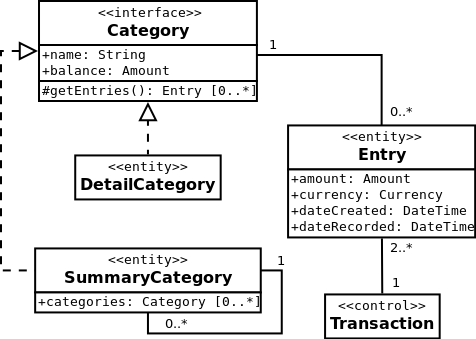
\includegraphics[width=11cm]{./contents/img/Class_Diagram_-_Summary_Category.png}
  \end{center}
  \caption{}
  \label{fig:ClassDiagram.SummaryCategory}
\end{figure}
\FloatBarrier

